\documentclass[TOTEM]{cern/cernphprep}

\def\d{{\rm d}}
\def\un#1{\,{\rm #1}}
\def\ung#1{\quad[{\rm #1}]}
\def\unt#1{[{\rm #1}]}
\def\e{{\rm e}}

\setbox123\hbox{\small$0$}
\def\S{\hbox to\wd123{\hss}}
\setbox124\hbox{\small$_{0}$}
\def\s{\hbox to\wd124{\hss}}

\def\etal{et al.}
\def\acknowledgments{\section*{Acknowledgements}}
\def\Name#1{\textsc{#1}, }
\def\REVIEW#1#2#3#4{{\it #1} {\bf #2} (#3) #4}

\def\Instline#1#2{%
	\expandafter\write1{\string\newlabel{#1}{{#1}{}}}%
	\hbox to\hsize{\strut\hss$^{#1}$#2\hss}
}

\def\hang{\hangindent=\parindent}
\catcode`\>=11
\newskip\itskip \itskip2mm
\newskip\iitskip \iitskip0mm
\newdimen\itindent \itindent3mm
\newdimen\iitindent \iitindent5mm
\def\>{\par\vskip\itskip\parindent\itindent\indent\hang\llap{\hbox to3mm{$\bullet$\hss}}}
\def\>E{\par\vskip\itskip\parindent\itindent\indent\hang\llap{\hbox to3mm{\hss}}}
\def\>>{\par\vskip\iitskip\parindent\iitindent\indent\hang\llap{\hbox to\iitindent{\hss--\ }}}



%----------------------------------------------------------------------------------------------------

\begin{document}

\begin{titlepage}

\renewcommand{\EXPLOGO}{fig/logo_totem_black.pdf}

\PHnumber{XXXX}
\PHdate{XXXX}

\EXPnumber{XXXX}
\EXPdate{XXXX}

%\title{Measurement of Elastic pp Scattering at $\sqrt{\hbox{s}} = \hbox{8}$\,TeV in the 
%Coulomb-Nuclear Interference Region by the TOTEM Experiment at the CERN LHC}

\title{TODO -- title}

\ShortTitle{TODO -- short title}

\Collaboration{The TOTEM Collaboration}
\ShortAuthor{The TOTEM Collaboration (G.~Antchev \emph{\etal})}

\begin{Authlist}
THIS IS JUST PLACEHOLDER -----------
G.~Antchev\Aref{a},
P.~Aspell\Iref{8},
I.~Atanassov\IAref{8}{a},
V.~Avati\Iref{8},
J.~Baechler\Iref{8},
V.~Berardi\IIref{5b}{5a},
M.~Berretti\Iref{7b},
E.~Bossini\Iref{7b},
M.~Bozzo\IIref{6b}{6a},
P.~Brogi\Iref{7b},
E.~Br\"{u}cken\IIref{3a}{3b},
A.~Buzzo\Iref{6a},
F.~S.~Cafagna\Iref{5a},
M.~Calicchio\IIref{5b}{5a},
M.~G.~Catanesi\Iref{5a},
C.~Covault\Iref{9},
M.~Csan\'{a}d\IAref{4}{e},
T.~Cs\"{o}rg\H{o}\Iref{4},
M.~Deile\Iref{8},
K.~Eggert\Iref{9},
V.~Eremin\Aref{b},
R.~Ferretti\IIref{6a}{6b},
F.~Ferro\Iref{6a},
A. Fiergolski\Aref{c},
F.~Garcia\Iref{3a},
S.~Giani\Iref{8},
V.~Greco\IIref{7b}{8},
L.~Grzanka\IAref{8}{d},
J.~Heino\Iref{3a},
T.~Hilden\IIref{3a}{3b},
R.~A.~Intonti\Iref{5a},
J.~Ka\v{s}par\IIref{1a}{8},
J.~Kopal\IIref{1a}{8},
V.~Kundr\'{a}t\Iref{1a},
K.~Kurvinen\Iref{3a},
S.~Lami\Iref{7a},
G.~Latino\Iref{7b},
R.~Lauhakangas\Iref{3a},
T.~Leszko\Aref{c},
E.~Lippmaa\Iref{2},
M.~Lokaj\'{\i}\v{c}ek\Iref{1a},
M.~Lo~Vetere\IIref{6b}{6a},
F.~Lucas~Rodr\'{i}guez\Iref{8},
M.~Macr\'{\i}\Iref{6a},
T.~M\"aki\Iref{3a},
A.~Mercadante\IIref{5b}{5a},
N.~Minafra\Iref{8} ,
S.~Minutoli\Iref{6a},
F.~Nemes\IAref{4}{e},
H.~Niewiadomski\Iref{8},
E.~Oliveri\Iref{7b},
F.~Oljemark\IAref{3a}{3b},
R.~Orava\IIref{3a}{3b},
M.~Oriunno\IAref{8}{f},
K.~\"{O}sterberg\IIref{3a}{3b},
P.~Palazzi\Iref{7b},
J.~Proch\'{a}zka\Iref{1a},
M.~Quinto\Iref{5a},
E.~Radermacher\Iref{8},
E.~Radicioni\Iref{5a},
F.~Ravotti\Iref{8},
E.~Robutti\Iref{6a},
L.~Ropelewski\Iref{8},
G.~Ruggiero\Iref{8},
H.~Saarikko\IIref{3a}{3b},
A.~Santroni\IIref{6b}{6a},
A.~Scribano\Iref{7b},
J.~Smajek\Iref{8},
W.~Snoeys\Iref{8},
J.~Sziklai\Iref{4},
C.~Taylor\Iref{9},
N.~Turini\Iref{7b},
V.~Vacek\Iref{1b},
M.~V\'itek\Iref{1b},
J.~Welti\IIref{3a}{3b} and
J.~Whitmore\Iref{10}
----------- END OF THE PLACEHOLDER
\end{Authlist}

\Instline{1a}{Institute of Physics of the Academy of Sciences of the Czech Republic, Praha, Czech Republic.}
\Instline{1b}{Czech Technical University, Praha, Czech Republic.}
\Instline{2} {National Institute of Chemical Physics and Biophysics NICPB, Tallinn, Estonia.}
\Instline{3a}{Helsinki Institute of Physics, Finland.}
\Instline{3b}{Department of Physics, University of Helsinki, Finland.}
\Instline{4} {MTA Wigner Research Center, RMKI, Budapest, Hungary.}
\Instline{5a}{INFN Sezione di Bari, Italy.}
\Instline{5b}{Dipartimento Interateneo di Fisica di Bari, Italy.}
\Instline{6a}{Sezione INFN, Genova, Italy.}
\Instline{6b}{Universit\`{a} degli Studi di Genova, Italy.}
\Instline{7a}{INFN Sezione di Pisa, Italy.}
\Instline{7b}{Universit\`{a} degli Studi di Siena and Gruppo Collegato INFN di Siena, Italy.}
\Instline{8} {CERN, Geneva, Switzerland.}
\Instline{9} {Case Western Reserve University, Dept. of Physics, Cleveland, OH, USA.}
\Instline{10}{Penn State University, Dept.~of Physics, University Park, PA, USA.}

\Anotfoot{a}{INRNE-BAS, Institute for Nuclear Research and Nuclear Energy, Bulgarian Academy of Sciences, Sofia, Bulgaria.}
\Anotfoot{b}{Ioffe Physical - Technical Institute of Russian Academy of Sciences.}
\Anotfoot{c}{Warsaw University of Technology, Poland.}
\Anotfoot{d}{Institute of Nuclear Physics, Polish Academy of Science, Cracow, Poland.}
\Anotfoot{e}{Department of Atomic Physics, E\"otv\"os University, Hungary.}
\Anotfoot{f}{SLAC National Accelerator Laboratory, Stanford CA, USA.}

\newpage

\begin{abstract}
TODO - abstract
\end{abstract}
\end{titlepage}


%----------------------------------------------------------------------------------------------------
\section{Introduction}

\> new: high-statistics data sample (same fill as DS2 from \cite{prl111}).
\>> eventually beyond dip/bumb
\>> for the moment only what is relevant for extrapolations to $t=0$

SOMEWHERE: x = horizontal, y = vertical

%----------------------------------------------------------------------------------------------------
\section{Experimental apparatus}

Detailed description elsewhere \cite{totem-jinst} - TODO, focus on RPs 220m only
\> structure: 2 arms, near and far units, 2 diagonals, ...

\> Minimal description of optics -- or in later sections ??

%----------------------------------------------------------------------------------------------------
\section{Data taking}

July 2012,
fill 2836,
$9.5\,\sigma_{\rm beam}$,
2 bunches in the beginning, later (when rate decreased) one more added,
TODO - typical bunch population,
TODO - typ. inst. luminosity,
$\beta^* = 90\un{m}$,
trigger settings (also mention zero-bias data),
little over $11\un{h}$ of data taking,
$735\un{\mu b^{-1}}$,
$7.2\cdot 10^6$ tagged elastic events,
minimal $|t| = 0.027\un{GeV^2}$ % left edge of left most bin


%----------------------------------------------------------------------------------------------------
\section{Analysis}

\> diagonals analysed separately, some steps done independent between bunches


%--------------------------------------------------
\subsection{Event reconstruction}

\begin{equation}
\label{eq:t}
t = p^2 ({\theta_x^*}^2 + {\theta_y^*}^2)
\end{equation}
TODO: projections of scattering angle

One-arm reconstruction -- minimise uncertainties due to optics imperfections
\begin{equation}
\label{eq:kin 1a}
\theta_x^* = {v_x^{\rm N} x^{\rm F} - v_x^{\rm F} x^{\rm N}\over v_x^{\rm N} L_x^{\rm F} - v_x^{\rm F} L_x^{\rm N}}\ ,\qquad
\theta_y^* = {1\over 2} \left( {y^{\rm N}\over L_y^{\rm N}} + {y^{\rm F}\over L_y^{\rm F}} \right)\ ,\qquad
x^* = {L_x^{\rm N} x^{\rm F} - L_x^{\rm F} x^{\rm N}\over L_x^{\rm N} v_x^{\rm F} - L_x^{\rm F} v_x^{\rm N}}
\end{equation}
x formula -- suppresses the impact of vertex.
Double-arm reconstruction
\begin{equation}
\label{eq:kin 2a}
\theta_x^* = (\theta_x^{*L} + \theta_x^{*R})/2\ ,\quad \theta_y^* = (\theta_y^{*L} + \theta_y^{*R})/2\ .
\end{equation}


Single arm for cuts, double-arm for physics.

{\bf Alignment}. Standard three-step procecure, details \cite{totem-ijmp}. Uncertainty: shifts $2\un{\mu m}$ (horizontal), $100\un{\mu m}$ (vertical) and rotations $0.2\un{mrad}$ (for each unit -- common for top and bottom RPs). Impact on angles (double-arm), horizontal shift $0.8\un{\mu rad}$, vertical shift $0.2\un{\mu rad}$ (effect disappears when diagonals combined). % rotation th_x^reco = th_x^true + A * th_y, si[A] = 0.02

{\bf Optics}. Matching \cite{totem-optics}, before: scale uncertainty (double-arm) $0.48\un{\%}$ (hor), $0.90\un{\%}$ (ver). After: scale uncertainty $0.21\un{\%}$ (hor), $0.25\un{\%}$ (ver) -- including the harmonics (not before). [not so spectacular difference: formula chosen to minimise the impact].

{\bf Resolutions} Beyond systematic uncertainties mentioned above, there are also statistical fluctuations -- beam divergence and for horizontal projection also detector resolution (low Lx). The resolutions can be experimentaly inferred from differences of the scattering angles determined from the left and right arms. Assuming identical resolutions in both arms, the standard deviation of the left-right difference is double of the angular resolution, see Eq.~(\ref{eq:kin 2a}). The resolutions were monitored in time to account for possible beam deterioation. The resolution in $\theta_y^*$ decreased from $1.6$ to $1.7\un{\mu rad}$ from the beginning to the end of the fill (DS3+DS4), for $\theta_x^*$ from $4.6$ to $4.8\un{\mu rad}$ (45b -- 56t) and from $4.3$ to $4.4\un{\mu rad}$ (45t -- 56b). In fact, just means over all bunches -- in analysis bunches treated independently. Comparing x and y, the contribution from the RP spatial resolution is evident. A cross check, horizontal beam div. from vertex distribution (sigma 145 to 185 urad, diagonal independent) % 2.3 to 2.9 urad
, the sensor contribution (2-arm) is $4.3$ (45b) and $4.0$ urad (45t), time independent. With the same method, not only RMS, but also shape. Generally, gaussian-like, with non-gaussianity decreasing with time. Non-gaussianinty taken accounted in systematic uncertainties. The original assumption of identical resolutions in both arms can be verified by checking the beam emittances. They give beam divergences compatible with our observations and indicate that a possible left-right imbalance could be of order $15\un{\%}$, which is used for uncertainty estimation.
TODO: why needed -- resolutions used in later steps

%--------------------------------------------------
\subsection{Differential cross-section}

For a given $t$ bin, the value of differential cross-section is evaluated by selecting and counting elastic events as follows
\begin{equation}
{\d\sigma\over \d t}(\hbox{bin}) =
	{\cal N}\, {\cal U}({\rm bin})\, {\cal B}\ 
	{\sum\limits_{t \in \hbox{bin}} {\cal A}(\theta_x^*, \theta_y^*)\, {\cal E}(\theta_y^*)\over \Delta t}\ ,
\end{equation}
where $\Delta t$ is the width of the bin, ${\cal N}$ is a normalisation factor and the other symbols stand for various correction factors:
 ${\cal U}$ for unfolding, ${\cal B}$ for backround subtraction, ${\cal A}$ for acceptace correction and ${\cal E}$ for detection and reconstruction efficiency.

{\bf Tagging}. The cuts used to select the elastic events are summarized in Tab.~\ref{tab:cuts}. Cuts 1 and 2 require the reconstructed-track collinearity between the left and right arm. Cuts 3 to 6 effectively work as low-$\xi$ cuts ($\xi$ being the fractional momentum loss of a proton).
Cuts 5 and 6: if $\xi\neq 0$, the correlation between the track position ($y^{\rm N}$) and the track angle (proportional to $y^{\rm F} - y^{\rm N}$) is lost. Cut 7 compares the horizontal vertex position reconstructed from the left and right arms. TODO: tagging inefficiency ? Aplly cuts at different sigmas. Difference between 4 and 5: about $0.5\un{\%}$, flat in $t$ (up to 0.2) thus irrelevant (due to the normalisation method).

\begin{table}
\caption{The elastic selection cuts. The superscripts R and L refer to the right and left arm, the N and F corresponds to the near and far units. The constant $\alpha = L_y^{\rm F} / L_y^{\rm N} - 1 \approx 0.107$. The right-most column gives the typical (there is diagonal and dataset dependence) RMS of the cut distribution ($\equiv 1\sigma$), all the cuts are applied at $4\sigma$-level.
}
\label{tab:cuts}
\begin{center}
\vskip-3mm
\begin{tabular}{ccc}\hline\hline
number & cut & RMS\cr\hline
diagonal &\multispan2 \hss track reconstructed in all 4 diagonal RPs \hss \cr
1 & $\theta_x^{*\rm R} - \theta_x^{*\rm L}$				& $9.5\un{\mu rad}$	\cr
2 & $\theta_y^{*\rm R} - \theta_y^{*\rm L}$				& $3.3\un{\mu rad}$	\cr
%3 & $|x^{*\rm R}|$ 										& $\un{\mu m}$	\cr
%4 & $|x^{*\rm L}|$ 										& $\un{\mu m}$	\cr
5 & $\alpha\,y^{\rm R,N} - (y^{\rm R,F} - y^{\rm R,N})$	& $18\un{\mu m}$	\cr
6 & $\alpha\,y^{\rm L,N} - (y^{\rm L,F} - y^{\rm L,N})$	& $18\un{\mu m}$	\cr
7 & $x^{*\rm R} - x^{*\rm L}$							& $8.5\un{\mu m}$ 	\cr\hline\hline
\end{tabular}
\end{center}
\end{table}

{\bf Background}. Cut distributions studied under different cut combinations: no change in signal part (below 4 sigmas), heavy impact outside signal region. After applying all cuts (except the studied one) and smoothly interpolating into the signal region, the $B/(S+B)$ ratio is $\approx 10^{-4}$ (for th x, th y and vtx x cuts). ${\cal B} = 1$, anyway irrelevant due to the normalisation approach.

{\bf Acceptance correction}. Two detection limitations: detector shape (mostly the edge facing beam, small $|\theta_y^*|$) and LHC apertures (high $|\theta_y^*|$). Two mechnisms: $\phi^*$ and beam divergence. The latter correctable due to known resolution (above) the former simply geometrical correction -- the theoretically expectable $\phi^*$ symmetry is confirmed by the date in the observable region. TODO: formula for ${\cal A}$ ?? TODO: Uncertainties.

\iffalse
\begin{equation}
\label{acceptance}
{\cal A_{\rm sm}}(\theta_y^*)^{-1} = {1\over 2} \left(
	\mathop{\rm Erf} {\min(\theta_y^{*,R,max} - |\theta_y^*|, |\theta_y^*| - \theta_y^{*,L,min})\over \sigma^{1a}_{\theta_y^*}}
	- \mathop{\rm Erf} {\max(\theta_y^{*,R,min} - |\theta_y^*|, |\theta_y^*| - \theta_y^{*,L,max})\over \sigma^{1a}_{\theta_y^*}}
\right)
\end{equation}

\begin{equation}
\label{acceptance}
{\cal A_{\phi}}(\theta_y^*) = {
	2\pi\over 
	\hbox{arc length with $\theta_y^*$ between } \max(\theta_y^{*,L,min}, \theta_y^{*,R,min}) \hbox{ and } \min(\theta_y^{*,L,max}, \theta_y^{*,R,max})
}
\end{equation}
\fi


{\bf Efficiency corrections} include corrections for inefficiencies from various sources: trigger inefficiency ${\cal I}_{\rm trig}$, reconsctruction inefficiency ${\cal I}_{\rm det}$ and pile-up inefficiency ${\cal I}_{\rm PU}$ (RPs unable to resolve multiple tracks):

\begin{equation}
\label{efficiency}
{\cal E}(\theta_y^*) = {1\over 1 - {\cal I}_{\rm trig}} {1\over 1 - {\cal I}_{\rm det}(\theta_y^*)} {1\over 1 - {\cal I}_{\rm PU}}\ ,\quad
{\cal I}_{\rm det}(\theta_y^*) = \sum\limits_{i\in \rm RPs} {\cal I}^i_{3/4}(\theta_y^*) + 2 {\cal I}_{2/4}
\end{equation}

The trigger and pile-up inefficiencies are mentioned for completeness only, since they do not affect the distribution shape, their values are not relevant the presented analysis due to a different way of final normalisation. The efects were nevertheless studied with techniques used in previous publications yielding expectable results.

Detector efficiency. Standard technique: 3/4 for every RP (${\cal I} \approx 1\un{\%}$ near and $2.5\un{\%}$ far) and 2/4 (${\cal I} = 1.5\un{\%}$) for the nears. 3/4 studied as function of $\theta_y^*$ to disentangle efficiency from acceptance effects. Furthermore, due to high statistics, gentle efficiency decrease with increasing $|\theta_y^*|$ was observed and taken into account. Average slope of the decrease per RP was $80\un{rad^{-1}}$ with a typical uncertainty of $8\un{rad^{-1}}$ for DS4.

%Trigger efficiency. Zero-bias data stream, events tagged as elastic, look at the trigger flag.
%For example for DS2, at $95\un{\%}$ CL, ${\cal I}_{\rm trig} < 8\cdot10^{-4}$. Anyway irrelevant.

{\bf Unsmearing}. Apriory: small effect due to the good angular resolution (above). 2 iterations: fit, Monte-Carlo calculation of the effect, correction of the ds/dt. Correction $|1 - {\cal U}| < 3\un{\%}$

{\bf Normalisation}. TODO: ${\cal N}$, same integral between $|t| = 0.027$ and $0.083\un{GeV^2}$ wrt.~dataset 1 from \cite{prl111}. Leading uncertainty: lumi error from DS2 ($4.2\un{\%}$), transfer to DS4 negligible (few per-mille)

{\bf Binning} Up to $0.8\un{GeV^2}$ one smearing sigma.

{\bf TODO: Estimate of systematics} Acc. corr. due to non-gauss, L-R asymmetry, both few per-mille withing final data. TODO: list leading uncertainties -- link to Tab.~\ref{tab:data}: optics modes 1 and 2, beam momentum -- this what we can't improve further

%--------------------------------------------------
\subsection{Final data merging}

\> central values and systematics

\> statistical uncertainties for "ob" binning rescale by $1/1.17596$ -- TODO: why

%----------------------------------------------------------------------------------------------------
\section{Results}

\begin{table*}
\caption{The elastic differential cross-section determined in this analysis.
representative points \cite{lafferty94}, uncertainty due to different fit models negligible ($10^{-7}\un{GeV^2}$). 
TODO: optimise number of digits
}
\label{tab:data}
\begin{center}
\scriptsize
\setlength{\tabcolsep}{3.5pt}
\begin{tabular}{ccc@{\hskip10pt}ccccccc}
\hline
\hline
\multispan3\hss $|t|$ bin $\unt{GeV^2}$\hss & \multispan7\hss $\d\sigma/\d t \ung{mb/GeV^2}$ \hss \cr
left & right & repres. & value & stat.     & full.~syst. & norm. & optics   & optics   & beam\cr
edge & edge  & point   &       & unc.      & unc.        &       & mode 1   & mode 2   & momentum\cr
\hline
$0.027$ & $0.030$ & $0.029$ & $300.945$ & $0.612$ & $12.909$ & $12.890$ & $-0.473$ & $-0.260$ & $+0.254$ \cr
$0.030$ & $0.033$ & $0.032$ & $284.042$ & $0.554$ & $12.130$ & $12.113$ & $-0.495$ & $-0.214$ & $+0.204$ \cr
$0.033$ & $0.037$ & $0.035$ & $265.588$ & $0.506$ & $11.370$ & $11.355$ & $-0.484$ & $-0.172$ & $+0.157$ \cr
$0.037$ & $0.040$ & $0.038$ & $247.896$ & $0.465$ & $10.632$ & $10.618$ & $-0.472$ & $-0.133$ & $+0.114$ \cr
$0.040$ & $0.044$ & $0.042$ & $231.953$ & $0.430$ & $ 9.917$ & $ 9.904$ & $-0.459$ & $-0.097$ & $+0.074$ \cr
$0.044$ & $0.047$ & $0.046$ & $215.353$ & $0.398$ & $ 9.225$ & $ 9.213$ & $-0.446$ & $-0.064$ & $+0.038$ \cr
$0.047$ & $0.051$ & $0.049$ & $199.885$ & $0.369$ & $ 8.559$ & $ 8.546$ & $-0.431$ & $-0.034$ & $+0.005$ \cr
$0.051$ & $0.055$ & $0.053$ & $184.554$ & $0.342$ & $ 7.917$ & $ 7.905$ & $-0.416$ & $-0.007$ & $-0.024$ \cr
$0.055$ & $0.060$ & $0.057$ & $170.715$ & $0.318$ & $ 7.303$ & $ 7.290$ & $-0.400$ & $+0.017$ & $-0.050$ \cr
$0.060$ & $0.064$ & $0.062$ & $156.615$ & $0.295$ & $ 6.715$ & $ 6.703$ & $-0.383$ & $+0.038$ & $-0.072$ \cr
$0.064$ & $0.068$ & $0.066$ & $142.958$ & $0.274$ & $ 6.155$ & $ 6.142$ & $-0.366$ & $+0.056$ & $-0.091$ \cr
$0.068$ & $0.073$ & $0.071$ & $131.310$ & $0.254$ & $ 5.623$ & $ 5.610$ & $-0.348$ & $+0.072$ & $-0.107$ \cr
$0.073$ & $0.078$ & $0.076$ & $119.589$ & $0.236$ & $ 5.120$ & $ 5.106$ & $-0.330$ & $+0.084$ & $-0.120$ \cr
$0.078$ & $0.083$ & $0.081$ & $108.278$ & $0.218$ & $ 4.645$ & $ 4.631$ & $-0.312$ & $+0.095$ & $-0.131$ \cr
$0.083$ & $0.089$ & $0.086$ & $ 97.732$ & $0.202$ & $ 4.199$ & $ 4.184$ & $-0.294$ & $+0.102$ & $-0.138$ \cr
$0.089$ & $0.094$ & $0.091$ & $ 87.916$ & $0.186$ & $ 3.781$ & $ 3.766$ & $-0.275$ & $+0.108$ & $-0.143$ \cr
$0.094$ & $0.100$ & $0.097$ & $ 78.866$ & $0.172$ & $ 3.391$ & $ 3.376$ & $-0.257$ & $+0.112$ & $-0.146$ \cr
$0.100$ & $0.106$ & $0.103$ & $ 70.641$ & $0.158$ & $ 3.029$ & $ 3.014$ & $-0.239$ & $+0.114$ & $-0.146$ \cr
$0.106$ & $0.112$ & $0.109$ & $ 62.480$ & $0.145$ & $ 2.694$ & $ 2.678$ & $-0.221$ & $+0.114$ & $-0.145$ \cr
$0.112$ & $0.119$ & $0.115$ & $ 55.454$ & $0.133$ & $ 2.386$ & $ 2.369$ & $-0.204$ & $+0.112$ & $-0.142$ \cr
$0.119$ & $0.125$ & $0.122$ & $ 48.733$ & $0.122$ & $ 2.103$ & $ 2.086$ & $-0.187$ & $+0.110$ & $-0.138$ \cr
$0.125$ & $0.132$ & $0.129$ & $ 42.712$ & $0.111$ & $ 1.844$ & $ 1.828$ & $-0.171$ & $+0.106$ & $-0.132$ \cr
$0.132$ & $0.140$ & $0.136$ & $ 37.277$ & $0.102$ & $ 1.610$ & $ 1.594$ & $-0.155$ & $+0.101$ & $-0.126$ \cr
$0.140$ & $0.147$ & $0.143$ & $ 32.207$ & $0.092$ & $ 1.398$ & $ 1.382$ & $-0.140$ & $+0.096$ & $-0.119$ \cr
$0.147$ & $0.155$ & $0.151$ & $ 27.731$ & $0.084$ & $ 1.207$ & $ 1.191$ & $-0.126$ & $+0.091$ & $-0.111$ \cr
$0.155$ & $0.163$ & $0.159$ & $ 23.827$ & $0.076$ & $ 1.035$ & $ 1.021$ & $-0.094$ & $+0.086$ & $-0.102$ \cr
$0.163$ & $0.172$ & $0.168$ & $ 20.364$ & $0.072$ & $ 0.881$ & $ 0.870$ & $-0.058$ & $+0.079$ & $-0.094$ \cr
$0.172$ & $0.181$ & $0.176$ & $ 17.249$ & $0.067$ & $ 0.746$ & $ 0.736$ & $-0.030$ & $+0.073$ & $-0.085$ \cr
$0.181$ & $0.190$ & $0.185$ & $ 14.480$ & $0.063$ & $ 0.628$ & $ 0.619$ & $-0.008$ & $+0.066$ & $-0.077$ \cr
$0.190$ & $0.200$ & $0.195$ & $ 12.124$ & $0.059$ & $ 0.526$ & $ 0.517$ & $+0.005$ & $+0.060$ & $-0.069$ \cr
\hline
\hline
\end{tabular}
\end{center}
\end{table*}

\begin{figure}
\begin{center}
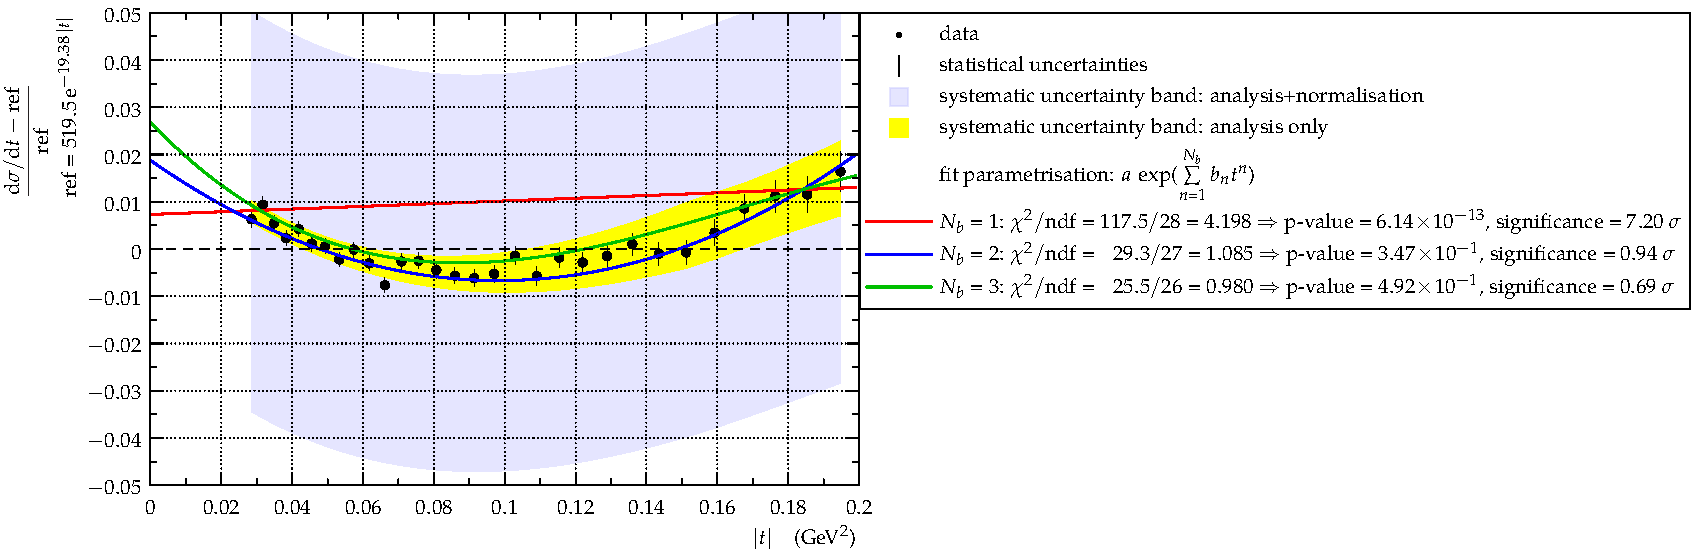
\includegraphics[width=18cm]{fig/t_dist_rel_with_fits.pdf}
\caption{TODO}
\label{fig:t dist rel}
\end{center}
\end{figure}


\> Describe exclusion of pure exponential - several methods

\> new determination of si tot?
\>> give values for "blue and green fits"

%----------------------------------------------------------------------------------------------------
\section{Discussion/Conclusions}

\> anything to add to the results section?

%----------------------------------------------------------------------------------------------------
\section{Outlook}

\> will extend this analysis beyond the dip
\> link to the $1000\un{m}$ paper?


%----------------------------------------------------------------------------------------------------
\acknowledgments

THIS IS JUST PLACEHOLDER -----------
We are indebted to the beam optics development team
%({\sc A.~Verdier} in the initial phase, {\sc H.~Burkhardt}, {\sc G.~M\" uller}, {\sc S.~Redaelli}, {\sc J.~Wenninger}, {\sc S.~M.~White})
for the design, the thorough preparations and the successful commissioning of the $\beta^* = 90\un{m}$ optics. We congratulate the CERN accelerator groups for the very smooth operation in 2011. We thank
%{\sc M.~Ferro-Luzzi}
the LHC machine coordinators for scheduling the dedicated fills.

This work was supported by the institutions listed on the front page and partially also by NSF (US), the Magnus
Ehrnrooth foundation (Finland), the Waldemar von Frenckell foundation (Finland), the Academy of
Finland, the OTKA grant NK 101438, 73143 (Hungary) and the NKTH-OTKA grant 74458 (Hungary).
----------- END OF THE PLACEHOLDER


%----------------------------------------------------------------------------------------------------
\begin{thebibliography}{99}

\bibitem{totem-jinst}
    %The TOTEM Experiment at the CERN Large Hadron Collider, JINST 3 S08007, 2008
	\Name{Anelli G.~\etal{}~(TOTEM Collaboration)}
	\REVIEW{JINST}{3}{2008}{S08007}

\bibitem{totem-ijmp}
	\Name{Antchev G.~\etal{}~(TOTEM Collaboration)}
	\REVIEW{Int.~J.~Mod.~Phys.~A}{28}{2013}{1330046}

\bibitem{totem-optics}
	\Name{Antchev G.~\etal{}~(TOTEM Collaboration)}
	LHC Optics Measurement with Proton Tracks Detected by the Roman Pots of the TOTEM Experiment, 
	arXiv:1406.0546

\bibitem{prl111}
	\Name{Antchev G.~\etal{}~(TOTEM Collaboration)}
	\REVIEW{Phys.~Rev.~Lett.}{111}{2013}{012001}

\bibitem{lafferty94}
 	% Where to stick your data points: The treatment of measurements within wide bins
	\Name{Lafferty G.~D.~and Wyatt T.~R.}
	\REVIEW{Nucl.\ Instrum.\ Meth.}{A 355}{1995}{541}


\iffalse

\bibitem{epl95}
    %Proton-proton elastic scattering at the LHC energy of \sqrt{s} = 7 TeV, Europhys. Lett. 95 (2011) 41001,CERN-PH-EP-2011-101 
	\Name{Antchev G.~\etal{}~(TOTEM Collaboration)}
	\REVIEW{Europhys.~Lett.}{95}{2011}{41001}

\bibitem{epl96}
    %First measurements of the total proton-proton cross-section at the LHC energy of $\sqrt s =7\,\rm TeV$ CERN-PH-EP-2011-158
	\Name{Antchev G.~\etal{}~(TOTEM Collaboration)}
	\REVIEW{Europhys.~Lett.}{96}{2011}{21002}

\bibitem{epl101-el}
	\Name{Antchev G.~\etal{}~(TOTEM Collaboration)}
	\REVIEW{Europhys.~Lett.}{101}{2013}{21002}

\bibitem{epl101-inel}
	\Name{Antchev G.~\etal{}~(TOTEM Collaboration)}
	\REVIEW{Europhys.~Lett.}{101}{2013}{21003}

\bibitem{epl101-tot}
	\Name{Antchev G.~\etal{}~(TOTEM Collaboration)}
	\REVIEW{Europhys.~Lett.}{101}{2013}{21004}

\bibitem{jan_thesis}
	\Name{Ka\v spar J.}
	PhD Thesis, CERN-THESIS-2011-214, {\tt http://cdsweb.cern.ch/record/1441140}

\bibitem{mario_ipac_2011}
	\Name{Deile M.}
	{\it The First 1 1/2 Years of TOTEM Roman Pot Operation at LHC}, in
	{\it Proceedings of the 2nd International Particle Accelerator Conference (IPAC 2011), San Sebastian, Spain}. 
	%{\tt http://accelconf.web.cern.ch/AccelConf/IPAC2011/papers/mopo011.pdf}
	arXiv:1110.5808v1

%\bibitem{pdg} 
%	\Name{Nakamura K.~\etal{} (Particle Data Group)}
%	\REVIEW{J.~Phys.}{G37}{2010}{075021}

\bibitem{B_vs_s}
	\Name{ISR (CR Collaboration)} \REVIEW{Phys.~Lett.}{B62}{1976}{460}; 
	\Name{ISR (ACHGT Collaboration)} \REVIEW{Phys.~Lett.}{B39}{1972}{663}; 
	\Name{ISR (R-211)} \REVIEW{Nucl.~Phys.}{B262}{1985}{689}; 
	\Name{ISR (R-210)} \REVIEW{Phys.~Lett.}{B115}{1982}{495}; 
	\Name{UA1} \REVIEW{Phys.~Lett.}{B147}{1984}{385}; 
	\Name{UA4} \REVIEW{Phys.~Lett.}{B127}{1983}{472} and \REVIEW{Phys. Lett.}{B198}{1987}{583}; 
	\Name{UA4/2} \REVIEW{Phys.~Lett.}{B316}{1993}{448}; 
	\Name{CDF} \REVIEW{Phys.~Rev.}{D50}{1994}{5518}; 
	\Name{E710} \REVIEW{Phys.~Rev.~Lett.}{68}{1992}{2433} and \REVIEW{Nuovo Cimento}{A106}{1992}{123}; 
	\Name{D0} D0 Note 6056-CONF; 
	\Name{pp2pp} \REVIEW{Phys.~Lett.}{B579}{2004}{245}

\bibitem{compete} 
	\Name{Cudell~J.~R.~\etal{} (COMPETE Collaboration)}
	\REVIEW{Phys.\ Rev.\ Lett.}{89}{2002}{201801}

\fi

\end{thebibliography}

\end{document}
